\newcommand{\Version}{0.001}

%%% Page formatting
%\setlength{\headsep}{30pt}
\setlength{\parindent}{25pt}
\setlength{\textheight}{9in}

%%% Header and Footer Info
\pagestyle{fancy}
\fancyhead[LO]{\small {\textbf{Antonius' Cookbook -- Version \Version}}}
\fancyhead[RE]{\small {\textbf{Antonius' Cookbook -- Version \Version}}}
\fancyhead[C]{}
\fancyhead[RO]{\small \thepage}
\fancyhead[LE]{\small \thepage}
\fancyfoot[L]{}
\fancyfoot[C]{}
\fancyfoot[R]{}


\patchcmd{\chapter}{plain}{empty}{}{}
\titleformat{\chapter}[display]
{\normalfont\huge\bfseries}{}{0pt}{\Huge}
\titlespacing*{\chapter} {0pt}{-50pt}{10pt}

%re-defines the plain page style
\fancypagestyle{plain}{%
	\fancyhf{}
	\rhead{\thepage}
	\renewcommand{\headrulewidth}{0pt}}

\newcommand\CoverPic{%
	\put(0,0){%
		\parbox[b][\paperheight]{\paperwidth}{%
			\vfill
			\centering
			{\transparent{0.3} 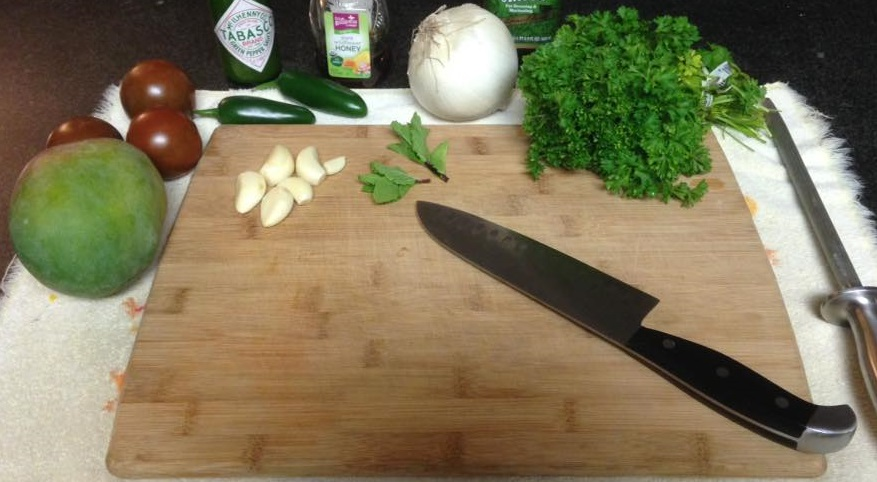
\includegraphics[height=\paperheight,%
				keepaspectratio]{./Images/CoverCropped.jpg}}%
			\vfill
}}}

\newcommand\Cheesecake{%
	\put(0,0){%
		\parbox[b][\paperheight]{\paperwidth}{%
			\vfill
			\centering
			{\transparent{0.3} 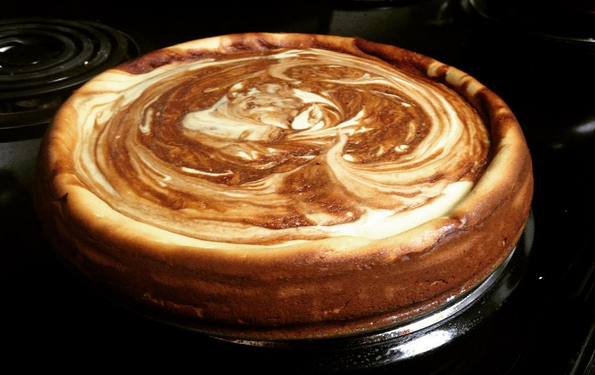
\includegraphics[height=\paperheight,%
				keepaspectratio]{./Images/MarbledCheesecake.png}}%
			\vfill
}}}

\newcommand\MexicanSoup{%
	\put(0,0){%
		\parbox[b][\paperheight]{\paperwidth}{%
			\vfill
			\centering
			{\transparent{0.3} 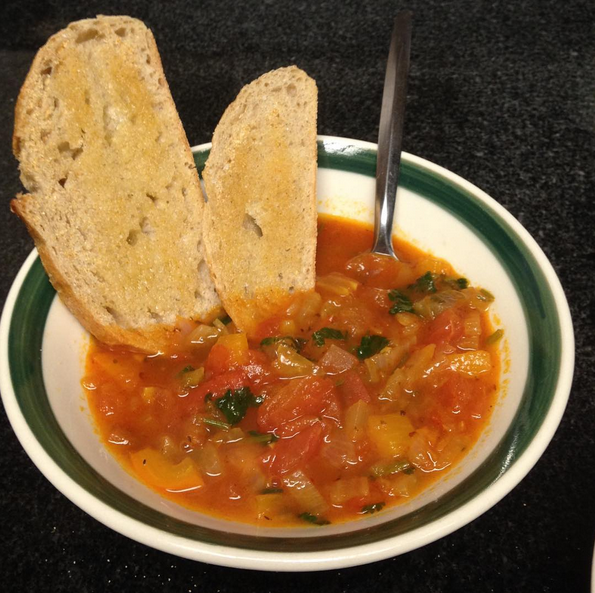
\includegraphics[height=\paperheight,%
				keepaspectratio]{./Images/SpicyMexicanSoup.png}}%
			\vfill
}}}

\newcommand\Calzone{%
	\put(0,0){%
		\parbox[b][\paperheight]{\paperwidth}{%
			\vfill
			\centering
			{\transparent{0.3} 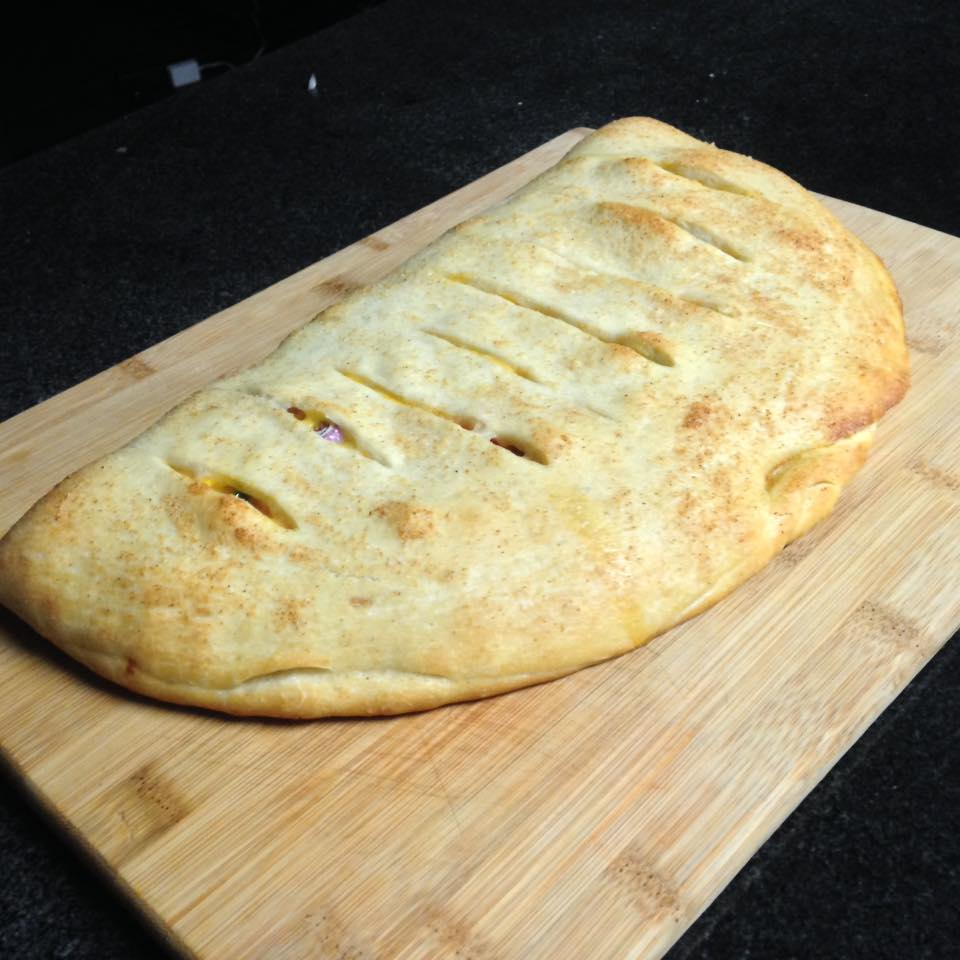
\includegraphics[height=\paperheight,%
				keepaspectratio]{./Images/Calzone.jpg}}%
			\vfill
}}}

\newcommand\CheesecakeTopping{%
	\put(0,0){%
		\parbox[b][\paperheight]{\paperwidth}{%
			\vfill
			\centering
			{\transparent{0.3} 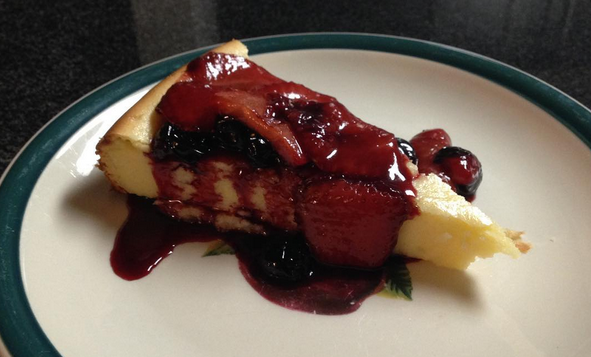
\includegraphics[height=\paperheight,%
				keepaspectratio]{./Images/CheesecakeTopping.png}}%
			\vfill
}}}

\newcommand\MangoSalsaTaco{%
	\put(0,0){%
		\parbox[b][\paperheight]{\paperwidth}{%
			\vfill
			\centering
			{\transparent{0.3} 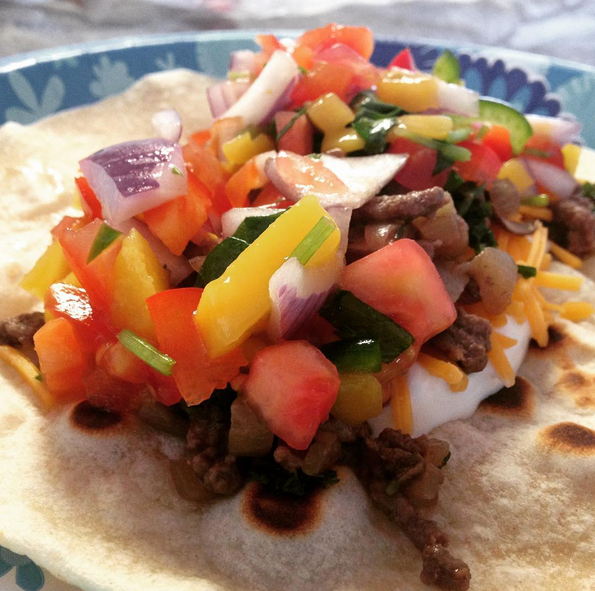
\includegraphics[height=\paperheight,%
				keepaspectratio]{./Images/MangeSalsaTacos.png}}%
			\vfill
}}}

\newcommand\EggSandwich{%
	\put(0,0){%
		\parbox[b][\paperheight]{\paperwidth}{%
			\vfill
			\centering
			{\transparent{0.3} 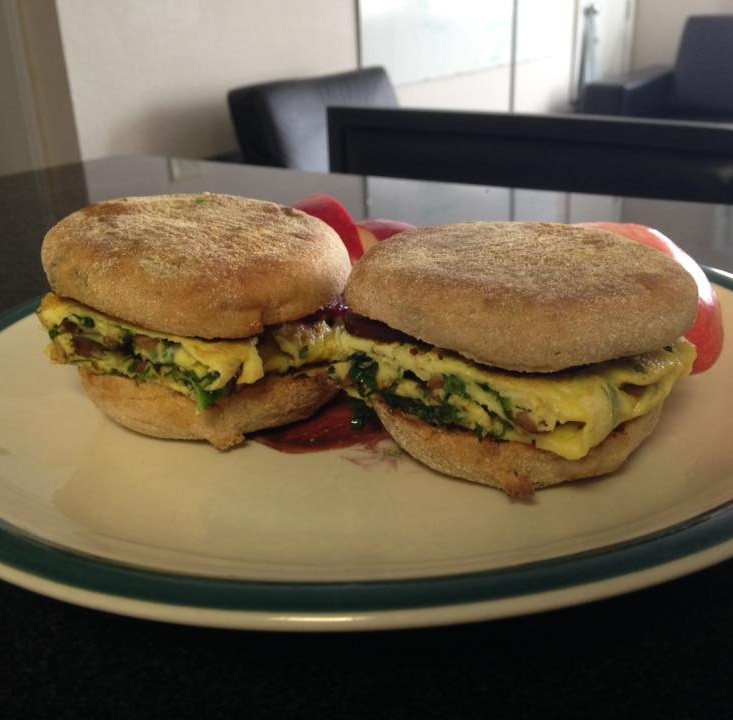
\includegraphics[height=\paperheight,%
				keepaspectratio]{./Images/EggSandwich.jpg}}%
			\vfill
}}}

\newcommand\AppleTart{%
	\put(0,0){%
		\parbox[b][\paperheight]{\paperwidth}{%
			\vfill
			\centering
			{\transparent{0.3} 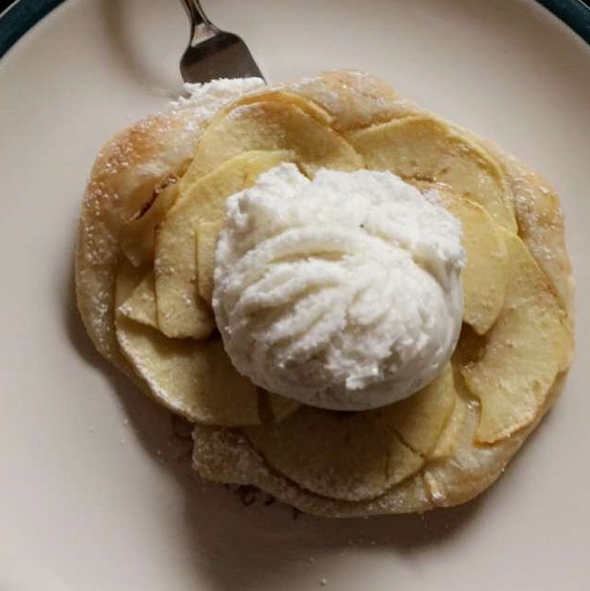
\includegraphics[height=\paperheight,%
				keepaspectratio]{./Images/AppleTartDesert.png}}%
			\vfill
}}}

\newcommand\MarinatedChickenAndRice{%
	\put(0,0){%
		\parbox[b][\paperheight]{\paperwidth}{%
			\vfill
			\centering
			{\transparent{0.3} 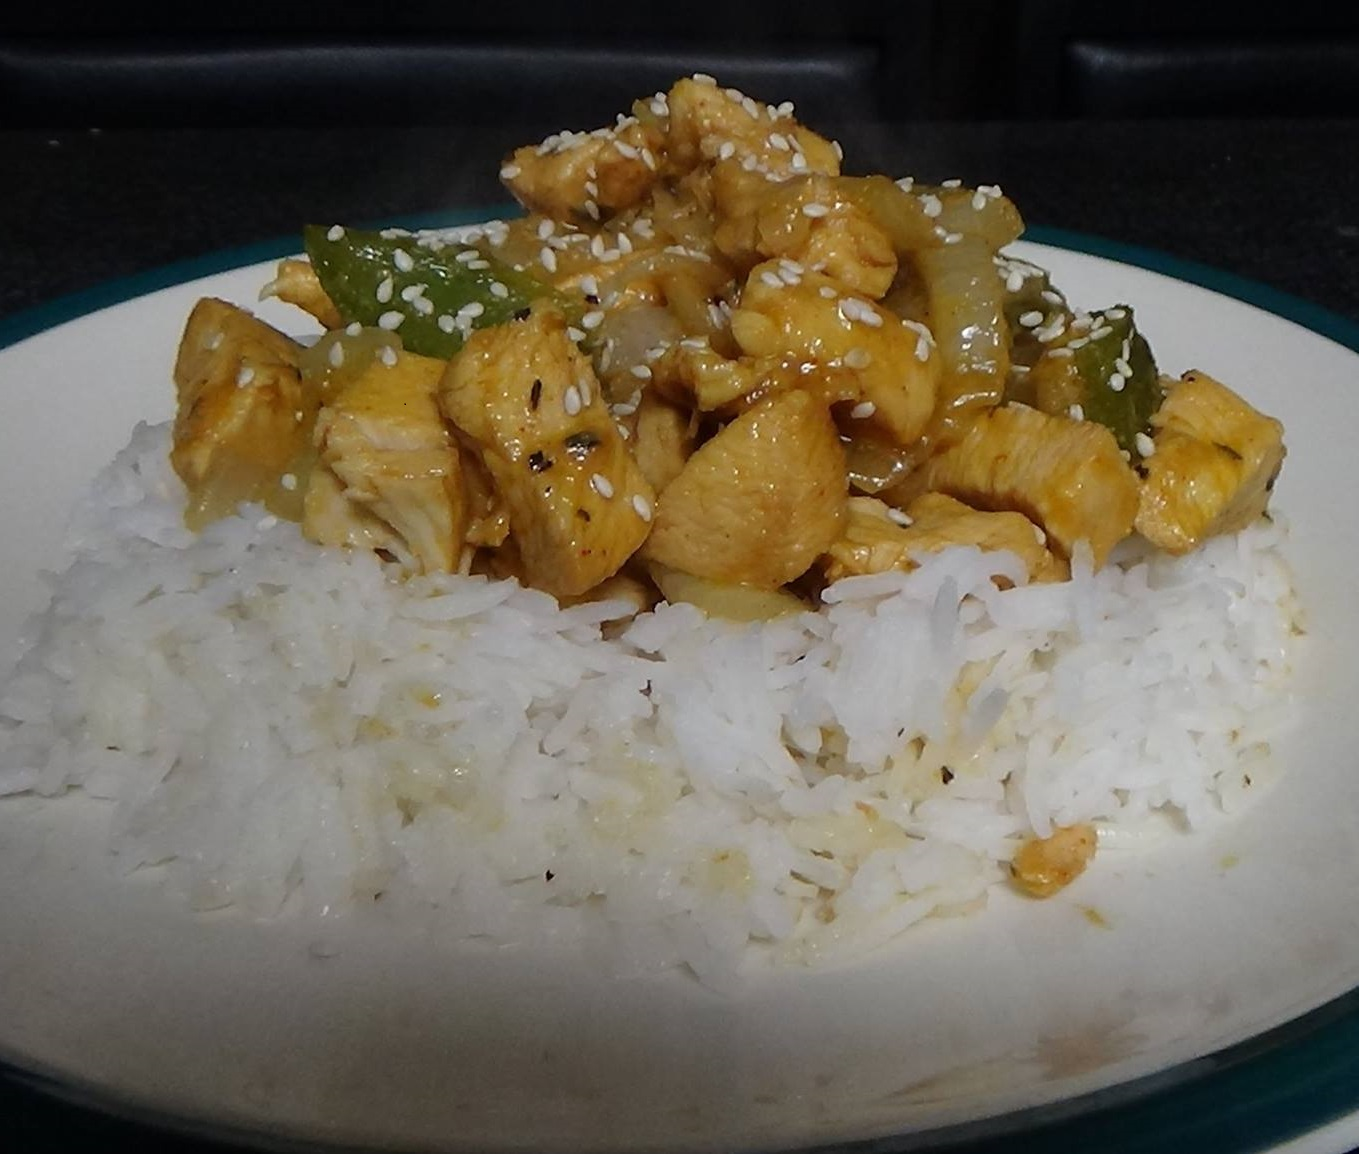
\includegraphics[height=\paperheight,%
				keepaspectratio]{./Images/chickenveggiesrice.jpg}}%
			\vfill
}}}

\newcommand\FetaSpinachEggs{%
	\put(0,0){%
		\parbox[b][\paperheight]{\paperwidth}{%
			\vfill
			\centering
			{\transparent{0.3} 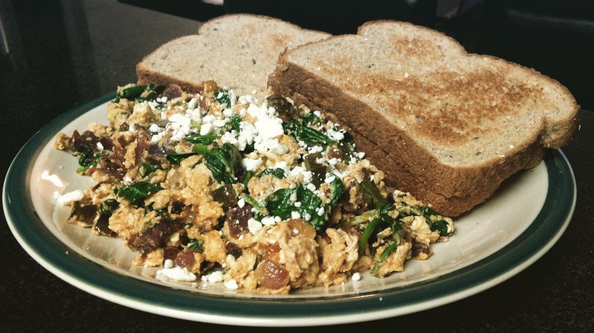
\includegraphics[height=\paperheight,%
				keepaspectratio]{./Images/FetaAndSpinachScrambledEggs.png}}%
			\vfill
}}}

\newcommand\StirFryRiceNoodles{%
	\put(0,0){%
		\parbox[b][\paperheight]{\paperwidth}{%
			\vfill
			\centering
			{\transparent{0.3} 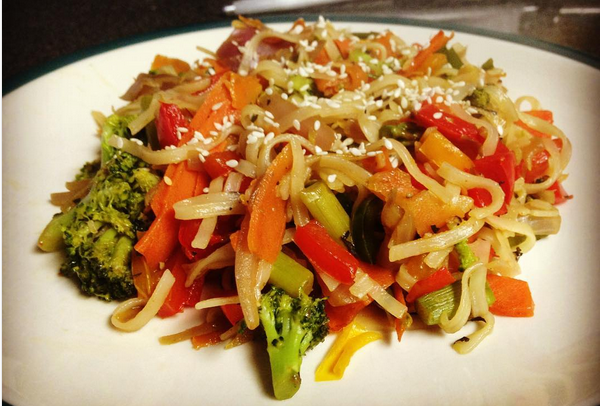
\includegraphics[height=\paperheight,%
				keepaspectratio]{./Images/StirFry_RiceNoodles.png}}%
			\vfill
}}}

\newcommand\Alfredo{%
	\put(0,0){%
		\parbox[b][\paperheight]{\paperwidth}{%
			\vfill
			\centering
			{\transparent{0.3} 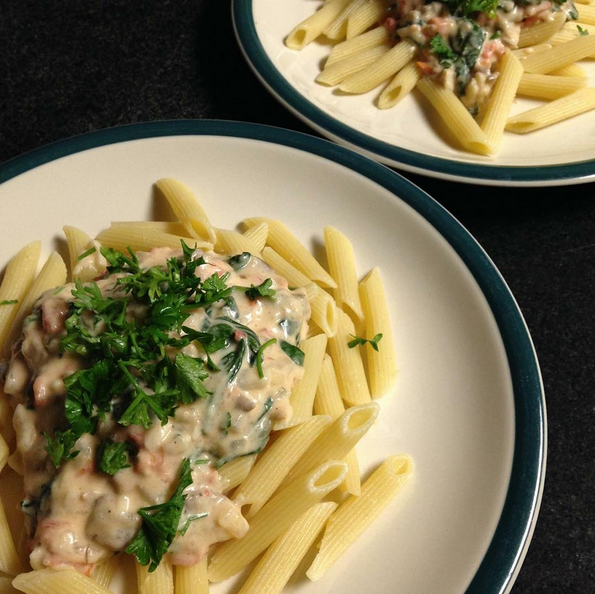
\includegraphics[height=\paperheight,%
				keepaspectratio]{./Images/Alfredo.png}}%
			\vfill
}}}

\newcommand\SteakAndEggs{%
	\put(0,0){%
		\parbox[b][\paperheight]{\paperwidth}{%
			\vfill
			\centering
			{\transparent{0.3} 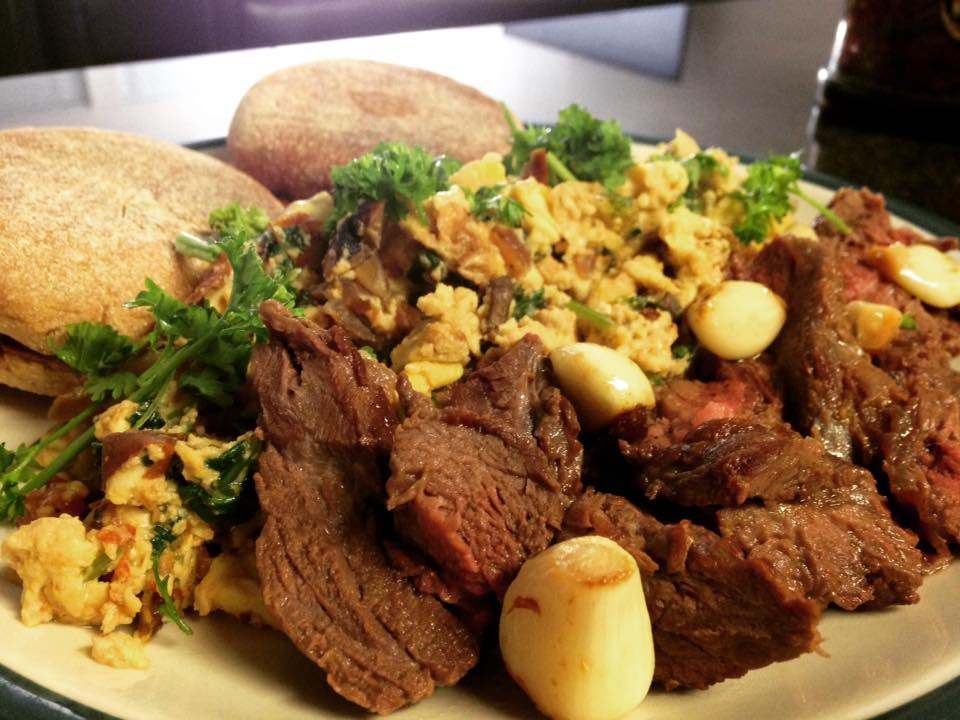
\includegraphics[height=\paperheight,%
				keepaspectratio]{./Images/SteakAndEggs.jpg}}%
			\vfill
}}}